	For the use of infrared thermography it can be found many studies for inspection application. The infrared camera makes it possible to work with thermal information in entire areas covered by the field of view, different from thermocouples which are able to measure punctual temperatures, for example.

	\citeonline{lee2011study} shows a study on integrity of resistance spot welding by means of infrared thermography. Two external heat sources were set in order to raise the temperature of the spot. The results have shown a promising method of inspection when it comes to diameter measurement of the nugget. While measurements made with naked eye provide an error about 20\%, the thermography provides only 8\%.

	Also \citeonline{lebar2010method} developed a method that allows online thermal measurement of abrasive water jet cutting. The method makes it possible to extract features from thermal image and to correlate them with texture analysis of the workpiece afterwards. This is important to evaluate the cutting process performance.

	\citeonline{abukhshim2006heat} summarized general methods for temperature measurement of the shear zone and tool-chip interface, but it points thermography methods to be the most suitable for high speed maching. There is no contact with the heat souces, preventing any external influences, in comparison with other methods, and the temperatures can be processed faster.	

	\begin{figure}[H]
		\centering
		\captionsetup{justification=centering}
		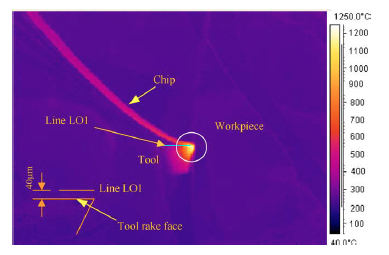
\includegraphics[scale=0.75]{Cap2/InfraRed/exinfrared.png}
		\caption{Infrared photography of a cutting process \cite{abukhshim2006heat}}
		\label{fig:exinfrared}
	\end{figure}

	For the case under study, high speed thermography has its positive and negative points. On the positive side, it may be mentioned:

	\begin{itemize}
		\item Fast inspection rate (reasonable number of images of high speed cutting)
		\item Contactless (no interference during the cutting process)
		\item Easy interpretation of the results (indexed image with temperatures in each pixel)
	\end{itemize}

	But it is also important to mention the difficulties that in this method still prevail:
	
	\begin{itemize}
		\item Only a limited thickness can be measured (under the main surface)
		\item Determiningl a suitable emissivity is a chalenge (it changes with temperature variation)
	\end{itemize}
